\section{Présentation des processus métiers}

\begin{description}
\item \bf{Offre et revue d'offre} : Un appel d'offre est lancé, donc une opportunité de contrat de service est saisie. Après analyse, ils peuvent faire suite ou non à cet appel d'offre. \\

\item \bf{Négociation client} : Ce processus n'est pour l'instant pas décrit, on le verra dans un second temps avec les axes d'amélioration. \\

\item \bf{Commande et revue de commande} : Si l'offre a été validée avec le client, il faut réaliser la revue du dossier de commande et négocier avec le client. \\

\item \bf{Lancement des prestations de service et travaux} : On lance la commande après qu'elle ait été accepté. Il faut mobiliser les ressources nécessaires et créer des documents opérationnels pour aboutir à une situation initiale connue. \\

\item \bf{Réalisation de prestations de maintenance} : Il faut exécuter les prestations mises en place. Une revue périodique de contrat est effectuée pour ensuite se diriger vers les évolutions du contrat. \\

\item \bf{Réalisation travaux induits} : On réalise tous les travaux éventuellement induits par ce qui a été effectué précédemment. S'il n'y en a pas, on passe à la suite. \\

\item \bf{\'Evolution du contrat} : Le contrat peut éventuellement évoluer après analyse des risques. \\

\item \bf{Solde de l'affaire et du contrat} : Une fois que tout a été effectué, on va clore le contrat et archiver tous les documents.
\end{description}

\section{Détail des différents processus}

\subsection{Offre et revue d'offre}

À la suite d'un appel d'offres, une opportunité de contrat de service est saisie. Il faut également réaliser une opportunité d'avenant, faisant sortir l'entreprise du cadre de maintenance corrective pour aller vers un cadre de maintenance évolutive. Le directeur opérationnel et le responsable d'activité maintenance décideront de la saisie de l'opportunité, tandis que le directeur opérationnel et le commercial donneront leur avis. S'ils décident de ne pas la saisir, le pilote de l'offre indiquera au client qu'ils ne souhaitent pas poursuivre. À l'inverse, si l'opportunité est saisie, il faut tout d'abord collecter des données (à la responsabilité du pilote de l'offre), puis les analyser avec l'aide éventuelle de la direction des ressources humaines et du service juridique (entres autres). \\

Après analyse, le pilote de l'offre peut décider de décliner la proposition et de confirmer au client que l'opportunité ne sera pas saisie. Dans le cas contraire, une réponse positive sera donnée au client. Il faut alors créer et enregistrer le dossier auprès du secrétariat de maintenance, puis proposer des solutions avec le calcul du prix de revient. Enfin, il faudra choisir la solution la plus adaptée ainsi et les prix de vente retenus. Il faut ensuite rédiger l'offre initiale et la faire valider en interne, pour finalement la transmettre dans les délais impartis.


\subsection{Commande et revue de commande}

Après avoir effectué la revue de l'offre, les négociations avec le client sont effectuées. Une fois l'offre validée avec le client, le secrétariat de maintenance l'enregistre et diffuse un original et des copies du dossier de commande. Le responsable d'activité maintenance affecte ensuite la commande au porteur opérationnel en désignant un responsable. Une fois la revue de commande effectuée, le responsable d'affaire valide les données nouvelles après avoir réalisé un plan d'action de validation. Il faut ensuite négocier avec le client, et les deux parties pourront soit trouver un accord et accepter la commande, soit la refuser s'ils n'arrivent pas à trouver un terrain d'entente. Quelle que soit l'issue de la négociation, le service commercial référence le contrat et son état.

\subsection{Lancement des prestations de service et travaux}

Si la commande a été acceptée, il faut la lancer. Les spécifications client sont connues, et on dispose de toutes les données internes nécessaires, le responsable d'affaire peut alors prendre en compte le dossier contractuel et le dossier d'étude. Le RA va alors analyser les exigences et les besoins, et identifier les acteurs afin de faire valider l'organigramme. \\

Une réunion de lancement a alors lieu, réunion pour laquelle seront présents tous les acteurs majeurs du contrat : RA, responsable opérationnel contrat (ROC), service des méthodes, mais aussi éventuellement les commerciaux, le service de gestion, ou encore la direction des ressources humaines, parmi d'autres. Une fois la réunion effectuée, il faut mobiliser les ressources nécessaires pour les rendre disponibles et opérationnelles, avec l'aide indispensable du ROC. En ayant à disposition le dossier de synthèse et les spécifications client, le ROC va créer des procédures et documents opérationnels. Le service des méthodes va alors initialiser des systèmes de gestion. Le responsable d'affaires reprend ensuite la main pour faire le bilan sur tous les actions et documents réalisés jusqu'à présent. Enfin, il va prendre en charge la situation afin d'aboutir à une situation initiale connue et maîtrisée.

\subsection{Réalisation de prestations de maintenance}

La commande de prestations de services et travaux est bien en place : il faut maintenant les exécuter, conformément à la commande et aux documents amonts, sous la responsabilité du responsable activité maintenance. \\

Mais il est également important de gérer l'affaire. Si on dispose de la commande initiale et que tous les documents amonts sont à la disposition du responsable d'affaires, alors la gestion de l'affaire débute dans l'objectif d'obtenir la maîtrise économique et juridique du contrat et de prévoir à nouveau la fin d'affaire. Le RA doit ensuite identifier les avenants (cf. revue d'offre) et les travaux induits (cf. sous-processus "réalisation travaux induits"). \\

Enfin, il faut gérer les activités et le reporting. En ayant à sa disposition les données issues des différents SI, on peut suivre les activités et le reporting client, puis effectuer une revue périodique de contrat grâce à cela, pour se diriger vers les évolutions du contrat.

\subsection{Réalisation travaux induits}

À la suite d'une demande faite par le client ou un intervenant du contrat, on souhaite réaliser des prestations de maintenance et identifier les travaux induits. En étudiant le cahier des charges, le responsable d'affaire va, avec l'aval du responsable opérationnel contrat, décider de donner suite ou non. S'ils décident de ne pas donner suite, il faut en informer le client. \\

Sinon, ils vont ensuite décréter si les travaux sous tous induits. Si ce n'est pas le cas, ces derniers seront redirigés vers le processus Travaux pour que tout soit prêt. Sinon, le RA et le ROC vont se demander si le contrat inclut les modalités d'exécution des travaux induits. Deux cas se présentent alors : \\
\begin{description}
\item Le contrat n'inclut pas les modalités d'exécution. Les travaux sont alors réalisés sur devis. Le RA et le ROC, avec l'aide éventuelle d'autres entités de la société, vont alors directement chiffrer, valider et envoyer ledit devis signé en fonction des pouvoirs. Une fois la commande reçue, elle est validée. \\

\item Le contrat inclut bien des modalités d'exécution. Les travaux sont alors réalisés en dépenses contrôlées, ou bien sur devis (suivant les clauses contractuelles). Le chiffrage et la validation des charges travaux sont ensuite effectués, puis le client est informé, ou on lui envoie un devis. Après réception de la commande orale ou de l'ordre de service, le RA va valider ceci et l'enregistrer sur Supra. \\
\end{description}

La préparation des travaux débute sous la responsabilité du responsable opérationnel contrat. Les consignes d'exécution sont remises au responsable de l'exécution avec les informations sur les éventuels risques et les mesures à prendre. L'exécution des prestations est effectuée, aboutissant à la mise à jour des documents d'exécution. Le client signe alors les documents reçus (PV de réception, CRI\dots), ce qui entraîne le déclenchement de la facture auprès du service Marché, ainsi que la gestion de la garantie.

\subsection{Évolution du contrat}

Grâce à la disponibilité du tableau de bord affaire et activités, des données comptables du système Supra et des différentes orientations (interne et client), le contrat peut évoluer sous la responsabilité du responsable d'affaire. Les risques sont analysés et un bilan de l'affaire est effectué. La décision est ensuite prise de renouveller l'affaire sous sa forme initiale ou sous une autre forme.

\subsection{Solde de l'affaire et du contrat}

L'affaire touche à sa fin : grâce à son bilan, la revue de contrat, les commandes et les avenants, il faut en effectuer la revue. Le client a pu constater des écarts par rapport à ce qui était prévu. Le RA va alors décider de solder les prestations et travaux et d'en effectuer une recette. \\

Un état des lieux de sortie est éventuellement réalisé sous la responsabilité du responsable opérationnel contrat. À la suite de cette réalisation, des écarts peuvent éventuellement être constatés, menant à un plan d'action. Il faut donc traiter ces écarts, et les solder en levant les réserves. \\

Grâce à la recette des prestations travaux et contrat, le responsable d'affaire peut gérer la garantie et en fermer le compte, déterminant la fin de la période de garantie. L'affaire peut alors être soldée et archivée.

\section{Description des données}

Commençons par souligner l’importance de quelques données capitales à la bonne gestion du processus de maintenance : \\

\begin{description}
\item \it{Données client :} Description du client, de son activité, ses coordonnées et diverses données à son propos.
\item \it{Devis :} Chiffrage de l’offre.
\item \it{Contrat :} Convention entre SPIE et son client.
\item \it{Offre :} Description globale de la solution proposée (ainsi que son détail) suite à une opportunité que l’équipe a saisie.
\end{description}

Cependant, il existe de nombreuses autres données nécessaires à ce processus.

\subsection{Données d’entrée}

\begin{table}[H]
    \centering
    \caption{Tableau descriptif des données d'entrée}
    \label{tab-donnees-entree}
    \begin{tabular}{p{5.5cm}|p{10cm}}
        \bf{Nom de la donnée d’entrée} & \bf{Description} \\ \hline
        Critères de décision & Regroupe l’ensemble des critères permettant de prendre une décision \\
        Opportunité de clientèle (PAC) & Plan d’actions commerciales lié à la clientèle de la société \\
        Climat concurrentiel & Conditions dans lesquelles s’exerce la concurrence \\
        Données collectées & Données collectées au début de la revue d’offre \\
        Compléments d'informations client & Informations supplémentaires liées au client \\
        Rapport d’analyse de risques & Rapport effectué à la suite de l’analyse des risques liés à l’offre \\
        Document de gestion des risques & Indique la façon dont les risques (juridiques, commerciaux, techniques\dots) seront gérés et est établi grâce aux données client notamment \\
        Courrier type de non-réponse & Courrier envoyé au client si l’offre ne sera pas poursuivie \\
        Règlement de consultation & Permet de constituer un dossier de réponse \\
        Dossier de réponse & Dossier envoyé au client suite à l’acceptation de l’offre \\
        Dossier d’étude & Dossier à propos de l’offre \\
        Données d’entreprise & Données liées à l’entreprise \\
        Mémoire technique type & \\
        Clauses contractuelles et juridiques & Clauses du contrat et de la justice de la filiale \\
        Clauses commerciales & Clauses mettant en lumière les dispositions particulières des deux parties concernées par l’offre \\
        Offre initiale & Offre lancée initialement par le client \\
        Courrier d’accompagnement & Courrier accompagnant la transmission de l’offre \\
        Dossier de commande & Dossier comprenant la commande \\
        Liste des écarts & Ecarts par rapport à la commande originale \\
        Plan d’action de validation & Plan d’action pour faire valider la commande \\
        Liste des réserves & Liste des points sur lesquels il y a désaccord \\ 
        Dossier contractuel & Dossier respectant le contrat \\
        Informations de référencement & Permettent au service commercial de référencer le dossier correctement \\
        Données internes & Consistuées de la QSE (Qualité Sécurité Environnement), documents de gestion, de RH\dots \\
        Dossier de synthèse & Comprend les exigences contractuelles \\
        Liste des ressources à mobiliser & Ressources présentant un intérêt pour l’affaire \\
        Organigramme contractuel & Organigramme des personnes en lien avec le contrat \\ 
        Planning du CR & Figure au compte-rendu de lancement \\
        Spécifications clients & Demandes particulières du client \\
        Rapport d’état des lieux & Rapport réalisé à la suite de l’état des lieux de la commande \\
        PV de prise en charge & Procès verbal nécessaire à la réalisation de la commande \\
        Commande de prestations & Prestations de service et travaux \\
        Avenant au contrat & Acte juridique apportant des modifications sur le contrat \\
        Travaux induits & Travaux supplémentaires induits par la commande \\
        PAQ & Plan d’Assurance Qualité \\
        Fiche d’ouverture de compte & \\
        Preuve de respect de l’engagement & Prouve l’engagement de moyens ou de la tenue du résultat \\
        PV de réception des travaux & Procès verbal poruvant la réception des travaux \\
        Sysnthèse des exigences client & Ensemble des demandes spécifiques effectuées par le client \\
        Cahier des charges & Cahier des charges des travaux induits \\
        Fiche devis vierge & Fiche de devis attendant d’être remplie \\
        Tableau de bord & Tableau de bord à propos de l’affaire et des différentes activités qui y sont liées \\
        Données comptables Supra & “Supra” est le système utilisé pour la comptabilité \\
        Bilan d’affaire & Bilan effectué à la suite d’une affaire menée à son terme afin de conserver un retour et éventuellement pouvoir reconduire l’affaire (avec ou sans modifications) \\
        Liste des écarts & Ecarts constatés par le client entre la commande initiale et le résultat \\
        CR état des lieux & Compte-rendu effectué à la suite de l’état des lieux de l’affaire \\
        PV état des lieux & Procès verbal effectué à partir du CR d’état des lieux \\
        Recette des prestations & Recette effectuée à partir des prestations travaux et du contrat
    \end{tabular}
\end{table}

\subsection{Données de sortie}

Nombre de données de sortie ont déjà été décrites dans les données d’entrée.

\begin{table}[H]
    \centering
    \caption{Tableau descriptif des données d'entrée}
    \label{tab-donnees-entree}
    \begin{tabular}{p{5.5cm}|p{10cm}}
        \bf{Nom de la donnée de sortie} & \bf{Description} \\ \hline
        Données collectées & Ensemble des données rassemblées pour décider si l’opportunité sera saisie \\
        Proposition de solution & Solution proposée au client pour son offre, avec un prix de revient \\
    Solution et prix de vente & Solution et prix retenus par le client et la société \\
        Données définitives & Données validées concernant l’affaire, incluant les réserves émises par le client \\
        Devis signé & Devis signé par le client et les personnes en pouvoir \\
        Documents d’exécution & Documents liés à la bonne réalisation des travaux induits (DOE, plans…)

    \end{tabular}
\end{table}

La figure suivante présente le modèle conceptuel de données décrivant les données existantes et les relations qu'elles ont entre elles.

\begin{figure}[H]
    \label{fig-mcd-existant}
    \noindent\makebox[\textwidth]{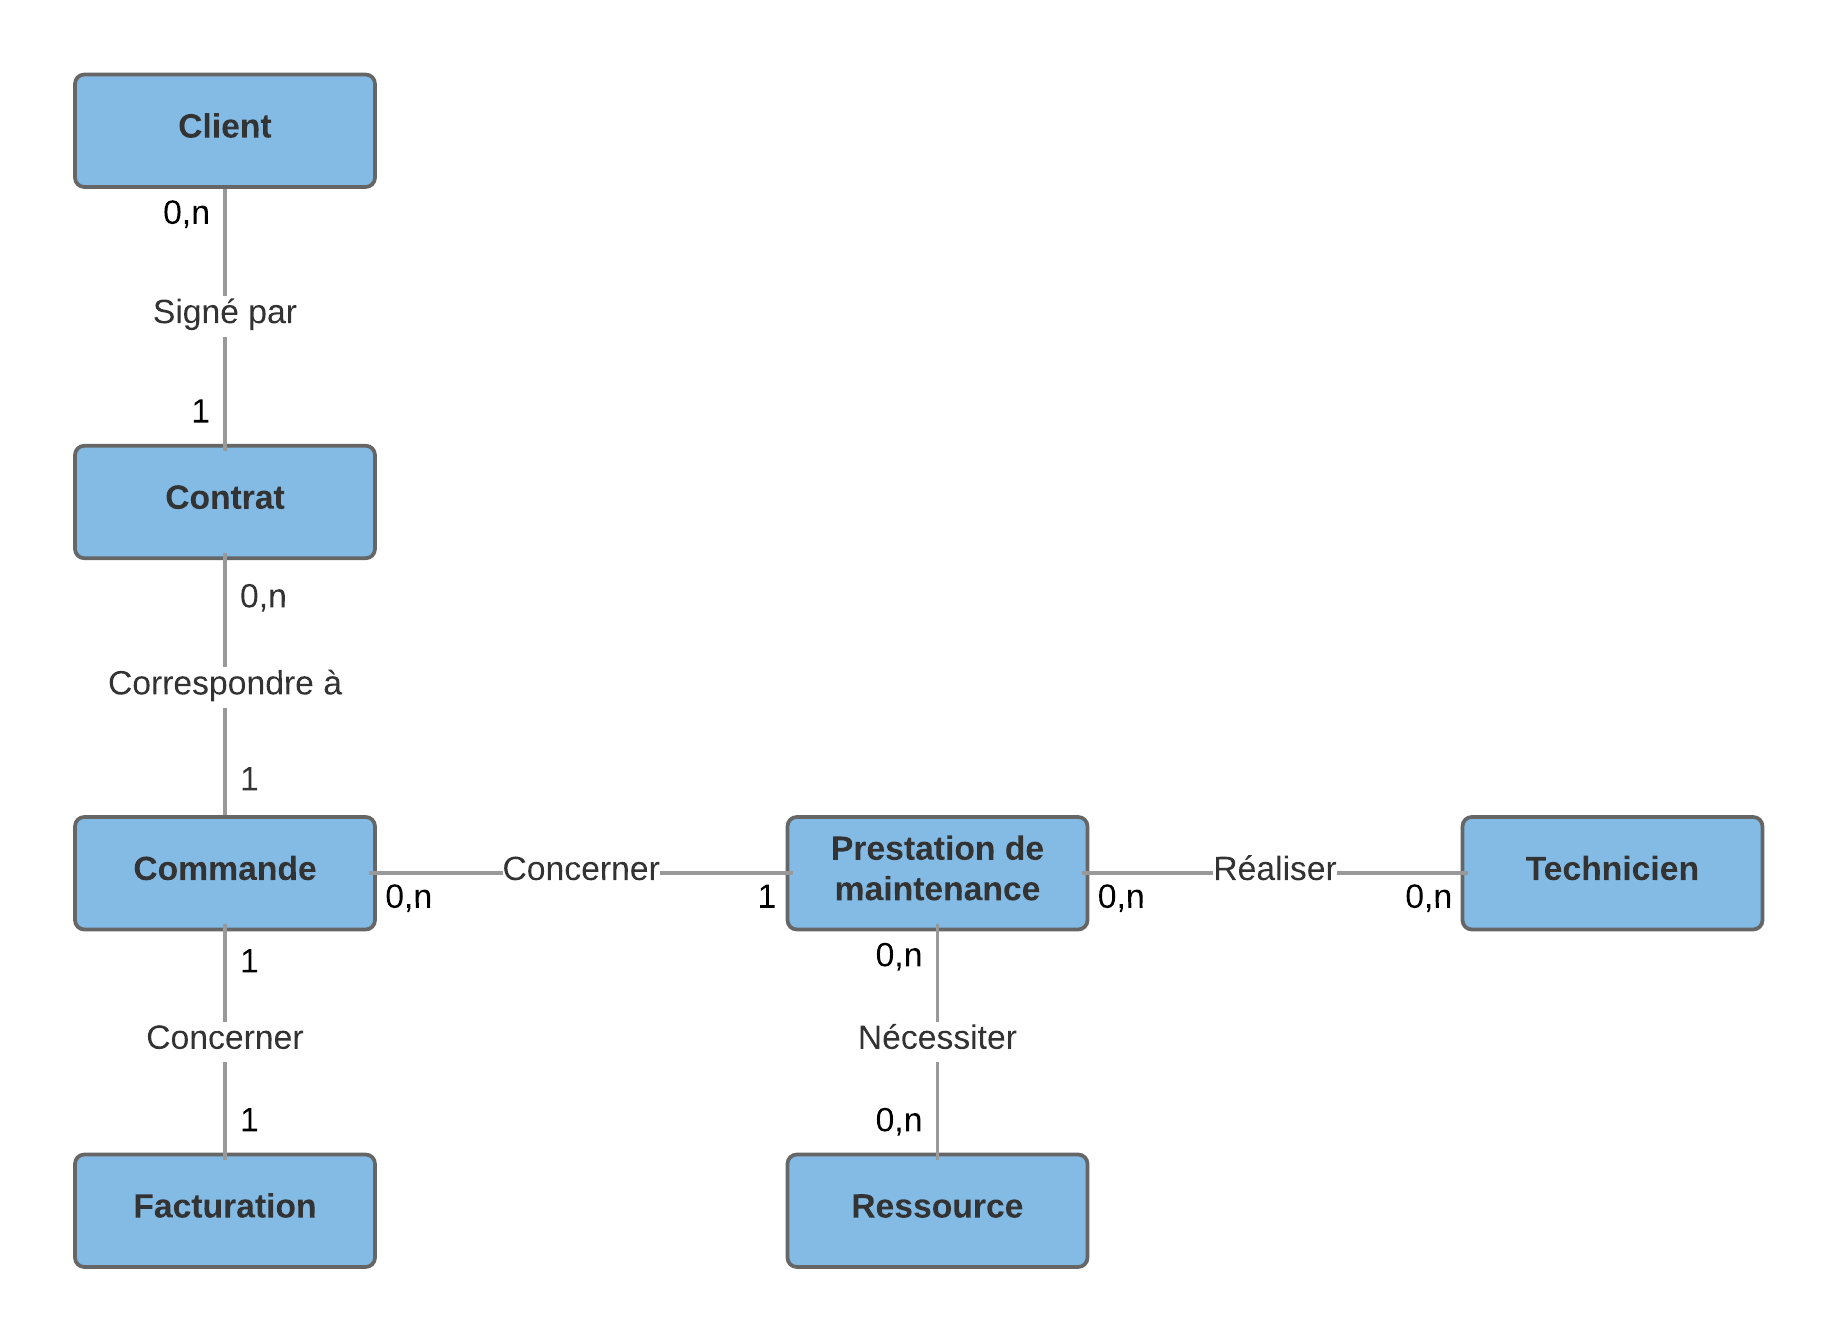
\includegraphics[width=15cm]{figures/mcd_existant.png}}
    \caption{MCD de l'existant}
\end{figure}

\section{Structure organisationnelle}

\begin{figure}[H]
    \label{fig-implem-spie}
    \noindent\makebox[\textwidth]{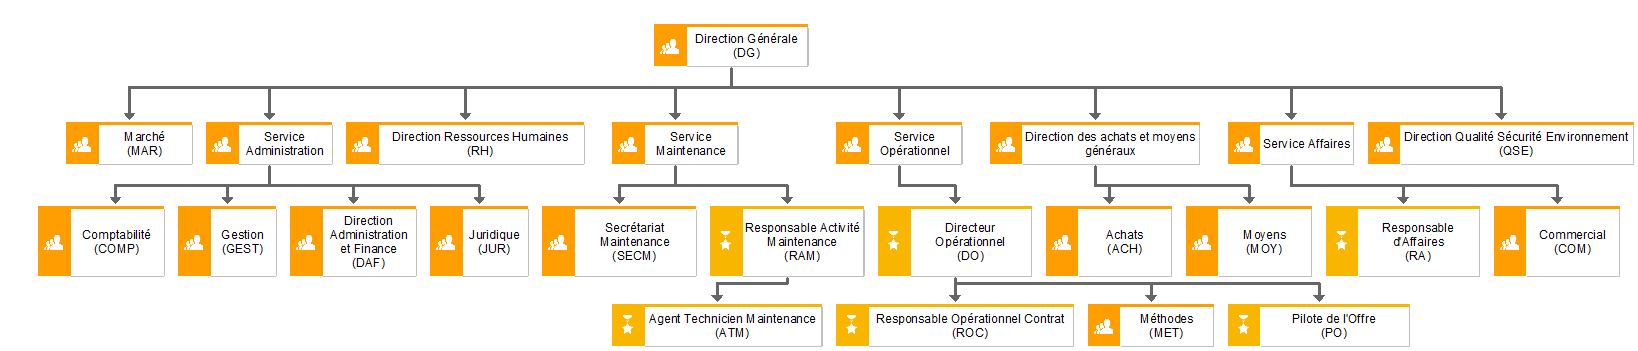
\includegraphics[width=25cm,angle=90]{figures/spie_organigramme.png}}
    \caption{Cartographie des implémentations de SPIE Sud-Est}
\end{figure}

